\documentclass[]{article}
\usepackage{lmodern}
\usepackage{amssymb,amsmath}
\usepackage{ifxetex,ifluatex}
\usepackage{fixltx2e} % provides \textsubscript
\ifnum 0\ifxetex 1\fi\ifluatex 1\fi=0 % if pdftex
  \usepackage[T1]{fontenc}
  \usepackage[utf8]{inputenc}
\else % if luatex or xelatex
  \ifxetex
    \usepackage{mathspec}
  \else
    \usepackage{fontspec}
  \fi
  \defaultfontfeatures{Ligatures=TeX,Scale=MatchLowercase}
\fi
% use upquote if available, for straight quotes in verbatim environments
\IfFileExists{upquote.sty}{\usepackage{upquote}}{}
% use microtype if available
\IfFileExists{microtype.sty}{%
\usepackage{microtype}
\UseMicrotypeSet[protrusion]{basicmath} % disable protrusion for tt fonts
}{}
\usepackage[margin=1in]{geometry}
\usepackage{hyperref}
\hypersetup{unicode=true,
            pdftitle={Example Rmarkdown Notebook},
            pdfauthor={Adam Lauretig},
            pdfborder={0 0 0},
            breaklinks=true}
\urlstyle{same}  % don't use monospace font for urls
\usepackage{color}
\usepackage{fancyvrb}
\newcommand{\VerbBar}{|}
\newcommand{\VERB}{\Verb[commandchars=\\\{\}]}
\DefineVerbatimEnvironment{Highlighting}{Verbatim}{commandchars=\\\{\}}
% Add ',fontsize=\small' for more characters per line
\usepackage{framed}
\definecolor{shadecolor}{RGB}{248,248,248}
\newenvironment{Shaded}{\begin{snugshade}}{\end{snugshade}}
\newcommand{\KeywordTok}[1]{\textcolor[rgb]{0.13,0.29,0.53}{\textbf{{#1}}}}
\newcommand{\DataTypeTok}[1]{\textcolor[rgb]{0.13,0.29,0.53}{{#1}}}
\newcommand{\DecValTok}[1]{\textcolor[rgb]{0.00,0.00,0.81}{{#1}}}
\newcommand{\BaseNTok}[1]{\textcolor[rgb]{0.00,0.00,0.81}{{#1}}}
\newcommand{\FloatTok}[1]{\textcolor[rgb]{0.00,0.00,0.81}{{#1}}}
\newcommand{\ConstantTok}[1]{\textcolor[rgb]{0.00,0.00,0.00}{{#1}}}
\newcommand{\CharTok}[1]{\textcolor[rgb]{0.31,0.60,0.02}{{#1}}}
\newcommand{\SpecialCharTok}[1]{\textcolor[rgb]{0.00,0.00,0.00}{{#1}}}
\newcommand{\StringTok}[1]{\textcolor[rgb]{0.31,0.60,0.02}{{#1}}}
\newcommand{\VerbatimStringTok}[1]{\textcolor[rgb]{0.31,0.60,0.02}{{#1}}}
\newcommand{\SpecialStringTok}[1]{\textcolor[rgb]{0.31,0.60,0.02}{{#1}}}
\newcommand{\ImportTok}[1]{{#1}}
\newcommand{\CommentTok}[1]{\textcolor[rgb]{0.56,0.35,0.01}{\textit{{#1}}}}
\newcommand{\DocumentationTok}[1]{\textcolor[rgb]{0.56,0.35,0.01}{\textbf{\textit{{#1}}}}}
\newcommand{\AnnotationTok}[1]{\textcolor[rgb]{0.56,0.35,0.01}{\textbf{\textit{{#1}}}}}
\newcommand{\CommentVarTok}[1]{\textcolor[rgb]{0.56,0.35,0.01}{\textbf{\textit{{#1}}}}}
\newcommand{\OtherTok}[1]{\textcolor[rgb]{0.56,0.35,0.01}{{#1}}}
\newcommand{\FunctionTok}[1]{\textcolor[rgb]{0.00,0.00,0.00}{{#1}}}
\newcommand{\VariableTok}[1]{\textcolor[rgb]{0.00,0.00,0.00}{{#1}}}
\newcommand{\ControlFlowTok}[1]{\textcolor[rgb]{0.13,0.29,0.53}{\textbf{{#1}}}}
\newcommand{\OperatorTok}[1]{\textcolor[rgb]{0.81,0.36,0.00}{\textbf{{#1}}}}
\newcommand{\BuiltInTok}[1]{{#1}}
\newcommand{\ExtensionTok}[1]{{#1}}
\newcommand{\PreprocessorTok}[1]{\textcolor[rgb]{0.56,0.35,0.01}{\textit{{#1}}}}
\newcommand{\AttributeTok}[1]{\textcolor[rgb]{0.77,0.63,0.00}{{#1}}}
\newcommand{\RegionMarkerTok}[1]{{#1}}
\newcommand{\InformationTok}[1]{\textcolor[rgb]{0.56,0.35,0.01}{\textbf{\textit{{#1}}}}}
\newcommand{\WarningTok}[1]{\textcolor[rgb]{0.56,0.35,0.01}{\textbf{\textit{{#1}}}}}
\newcommand{\AlertTok}[1]{\textcolor[rgb]{0.94,0.16,0.16}{{#1}}}
\newcommand{\ErrorTok}[1]{\textcolor[rgb]{0.64,0.00,0.00}{\textbf{{#1}}}}
\newcommand{\NormalTok}[1]{{#1}}
\usepackage{graphicx,grffile}
\makeatletter
\def\maxwidth{\ifdim\Gin@nat@width>\linewidth\linewidth\else\Gin@nat@width\fi}
\def\maxheight{\ifdim\Gin@nat@height>\textheight\textheight\else\Gin@nat@height\fi}
\makeatother
% Scale images if necessary, so that they will not overflow the page
% margins by default, and it is still possible to overwrite the defaults
% using explicit options in \includegraphics[width, height, ...]{}
\setkeys{Gin}{width=\maxwidth,height=\maxheight,keepaspectratio}
\IfFileExists{parskip.sty}{%
\usepackage{parskip}
}{% else
\setlength{\parindent}{0pt}
\setlength{\parskip}{6pt plus 2pt minus 1pt}
}
\setlength{\emergencystretch}{3em}  % prevent overfull lines
\providecommand{\tightlist}{%
  \setlength{\itemsep}{0pt}\setlength{\parskip}{0pt}}
\setcounter{secnumdepth}{0}
% Redefines (sub)paragraphs to behave more like sections
\ifx\paragraph\undefined\else
\let\oldparagraph\paragraph
\renewcommand{\paragraph}[1]{\oldparagraph{#1}\mbox{}}
\fi
\ifx\subparagraph\undefined\else
\let\oldsubparagraph\subparagraph
\renewcommand{\subparagraph}[1]{\oldsubparagraph{#1}\mbox{}}
\fi

%%% Use protect on footnotes to avoid problems with footnotes in titles
\let\rmarkdownfootnote\footnote%
\def\footnote{\protect\rmarkdownfootnote}

%%% Change title format to be more compact
\usepackage{titling}

% Create subtitle command for use in maketitle
\newcommand{\subtitle}[1]{
  \posttitle{
    \begin{center}\large#1\end{center}
    }
}

\setlength{\droptitle}{-2em}
  \title{Example Rmarkdown Notebook}
  \pretitle{\vspace{\droptitle}\centering\huge}
  \posttitle{\par}
  \author{Adam Lauretig}
  \preauthor{\centering\large\emph}
  \postauthor{\par}
  \predate{\centering\large\emph}
  \postdate{\par}
  \date{\today}

\usepackage{palatino}
\usepackage{graphicx}
\usepackage{scrextend}

\begin{document}
\maketitle

\subsection{R Markdown}\label{r-markdown}

This is an R Markdown document. Markdown is a simple formatting syntax
for authoring HTML, PDF, and MS Word documents. For more details on
using R Markdown see \url{http://rmarkdown.rstudio.com}. To produce the
output, click ``Knit'', next to the magnifying glass.

When you click the \textbf{Knit} button a document will be generated
that includes both content as well as the output of any embedded R code
chunks within the document. You can embed an R code chunk like this:

\begin{Shaded}
\begin{Highlighting}[]
\KeywordTok{summary}\NormalTok{(cars)}
\end{Highlighting}
\end{Shaded}

\begin{verbatim}
##      speed           dist       
##  Min.   : 4.0   Min.   :  2.00  
##  1st Qu.:12.0   1st Qu.: 26.00  
##  Median :15.0   Median : 36.00  
##  Mean   :15.4   Mean   : 42.98  
##  3rd Qu.:19.0   3rd Qu.: 56.00  
##  Max.   :25.0   Max.   :120.00
\end{verbatim}

When you examine the chunk, you see that the first line has several
things going on. You can generate a new chunk with It begins with ```,
which marks the beginning of a code chunk. You can create your own new
code chunk by clicking ``insert,'' and then selecting \texttt{R}. The
chunk first tells you that it is \texttt{r} code, then has a name,
``cars.'' I would recommend giving your code chunks informative names,
and making sure these names are unique. \texttt{cache\ =\ TRUE} tells R
to save the results, so that once we run the code once, we won't have to
re-run it every time (as long as we don't change anything).

If we don't want our code chunk to be visible (we only want to see the
results), we can include another flag in the header,
\texttt{echo\ =\ FALSE}, which tells R to run the code, but to only
display the results.

\begin{verbatim}
##      speed           dist       
##  Min.   : 4.0   Min.   :  2.00  
##  1st Qu.:12.0   1st Qu.: 26.00  
##  Median :15.0   Median : 36.00  
##  Mean   :15.4   Mean   : 42.98  
##  3rd Qu.:19.0   3rd Qu.: 56.00  
##  Max.   :25.0   Max.   :120.00
\end{verbatim}

If we want to display code which we won't run (such as homework code
that you can't get to work, but include for partial credit), you can add
an \texttt{eval\ =\ FALSE} flag to your code chunk.

\begin{Shaded}
\begin{Highlighting}[]
\NormalTok{This code will not run. }
\end{Highlighting}
\end{Shaded}

Generally, for homework assignments, you will use the
\texttt{echo\ =\ FALSE} flag, and just display your output. You should
also use the \texttt{cache\ =\ TRUE} flag, so that you won't have to
re-run all of your code every time.

\subsection{Including Plots}\label{including-plots}

You can also embed plots, for example:

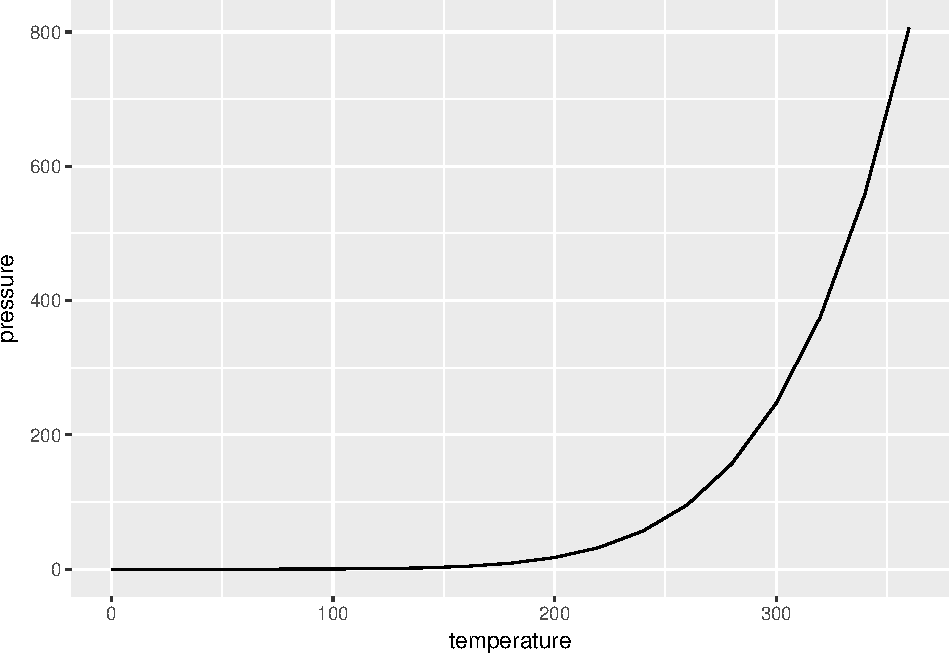
\includegraphics{example_rmarkdown_files/figure-latex/pressure-1.pdf}

We'll use \texttt{echo\ =\ FALSE}, so that we only see the plot.
However, we may want to add a caption to the image, so that we can
describe what we'll see. We can put this in the header:

\begin{figure}[htbp]
\centering
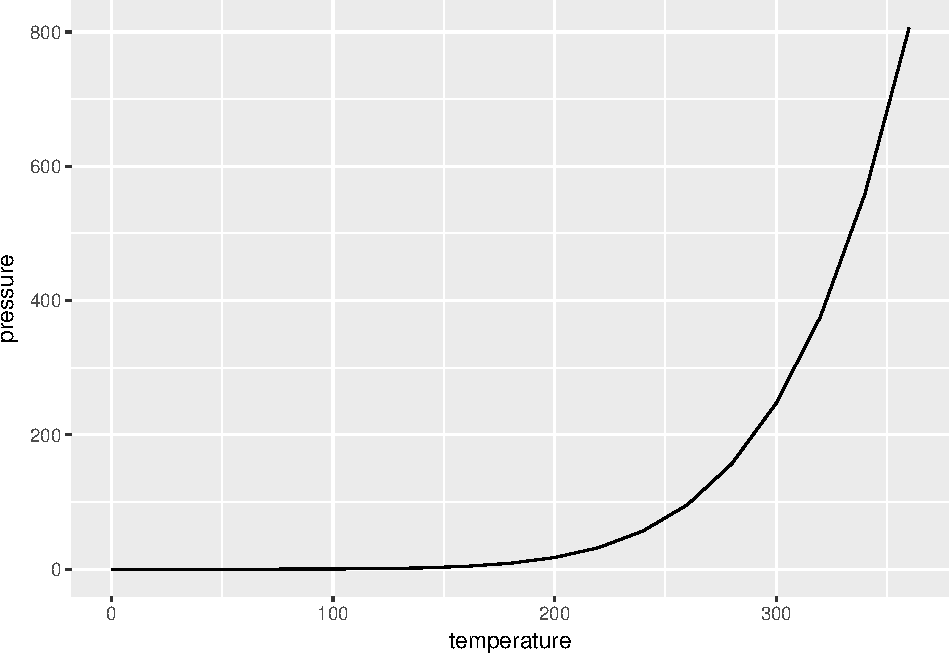
\includegraphics{example_rmarkdown_files/figure-latex/pressure_cap-1.pdf}
\caption{Plotting Temperature vs.~Pressure}
\end{figure}

But this figure is pretty big. We can adjust the size with a few more
flags in the header. Using \texttt{fig.width\ =\ 3,\ fig.height=\ 2},
we'll tell \texttt{R} we want a \(4\times3\) inch figure for our plot.

\begin{figure}[htbp]
\centering
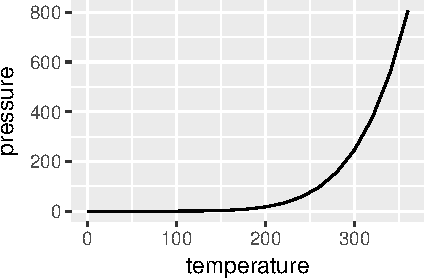
\includegraphics{example_rmarkdown_files/figure-latex/pressure_cap_size-1.pdf}
\caption{Plotting Temperature vs.~Pressure}
\end{figure}

We can include links to figures in the text of the document, which is
helpful when writing analysis, we'll add text to the caption, so that we
can reference figure \ref{fig:tp} . I also included
\texttt{fig.align=\textquotesingle{}center\textquotesingle{},\ fig.show=\textquotesingle{}hold\textquotesingle{}}
in the header, so that the figure would stay centered (which is not
necessary, but aesthetically, I like it.)

\begin{figure}

{\centering 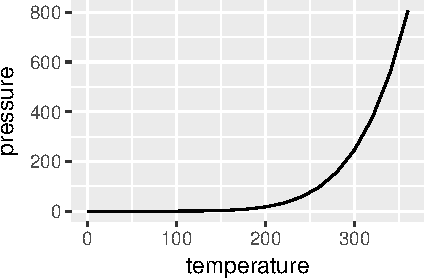
\includegraphics{example_rmarkdown_files/figure-latex/pressure_cap_size_ling-1} 

}

\caption{\label{fig:tp}Plotting Temperature vs. Pressure with a label}\label{fig:pressure_cap_size_ling}
\end{figure}

\newpage

\section{Writing out Math}\label{writing-out-math}

One additional reason to use \texttt{Rmarkdown} is that we can use the
Latex engine underneath it to write out nice looking math, which saves
the trouble of having to figure out handwritten notes in a presentation.
For example, we can write out a regression equation as
\(y = \alpha + X\beta + \varepsilon\), without having to copy and past
anything in. To write out anything math related, we enclose it in dollar
signs \(\$\)\texttt{math}\(\$\). The regression example above, for
example, is \(\$\)
\texttt{y\ =\ \textbackslash{}alpha\ +\ X\textbackslash{}beta\ +\ \textbackslash{}varepsilon}
\(\$\). If we want to index something \(x_{1}, x_{2}\) etc, the code is
\(\$\)\texttt{x\_\{1\},\ x\_\{2\}}\(\$\). Fractions are written
\(\frac{1}{2}\), \(\$\)\texttt{\textbackslash{}frac\{1\}\{2\}}\(\$\),
and exponents (\(2^{2}\)) are written \(\$\)\texttt{2\^{}\{2\}}\(\$\).

You'll notice the greek letters have a slash before them, but the
letters don't. This slash tells Latex to print that as a greek letter.
Similarly \(2 \times 2\) is written \(\$\)
\texttt{2\ \textbackslash{}times\ 2} \(\$\). A useful guide to special
characters and formatting in Latex is here
\url{https://users.dickinson.edu/~richesod/latex/latexcheatsheet.pdf}. I
reference it fairly regularly.

\subsection{Matrices}\label{matrices}

To implement a matrix: \[ 
\left[
\begin{array}{ccc}
1 & 2 & 3 \\
4 & 5 & 6\\
7 & 8 & 0
\end{array}
\right] 
\] you'll need to write:

\begin{Shaded}
\begin{Highlighting}[]
\NormalTok{$}\ErrorTok{$}\StringTok{ }\NormalTok{% start Latex mode}
\NormalTok{\textbackslash{}left[ %creates the left bracket, the }\StringTok{"\textbackslash{}left"} \NormalTok{command scales the bracket }\StringTok{"["}
\NormalTok{\textbackslash{}begin\{array\}\{ccc\} % Creates the }\StringTok{"array"} \NormalTok{(matrix), \{ccc\} defines the number of columns}
\DecValTok{1} \NormalTok{&}\StringTok{ }\DecValTok{2} \NormalTok{&}\StringTok{ }\DecValTok{3} \NormalTok{\textbackslash{}\textbackslash{} % }\StringTok{"&"} \NormalTok{divides the columns, }\StringTok{"}\CharTok{\textbackslash{}\textbackslash{}}\StringTok{"} \NormalTok{creates a new line}
\DecValTok{4} \NormalTok{&}\StringTok{ }\DecValTok{5} \NormalTok{&}\StringTok{ }\DecValTok{6}\NormalTok{\textbackslash{}\textbackslash{}}
\DecValTok{7} \NormalTok{&}\StringTok{ }\DecValTok{8} \NormalTok{&}\StringTok{ }\DecValTok{0}
\NormalTok{\textbackslash{}end\{array\} % ends the matrix}
\NormalTok{\textbackslash{}right] %creates the left bracket, the }\StringTok{"}\CharTok{\textbackslash{}r}\StringTok{ight"} \NormalTok{command scales the bracket }\StringTok{"]"}
\NormalTok{$}\ErrorTok{$}\StringTok{ }\NormalTok{% ends Latex mode}
\end{Highlighting}
\end{Shaded}

without comments:

\begin{Shaded}
\begin{Highlighting}[]
\NormalTok{$}\ErrorTok{$}\StringTok{ }
\NormalTok{\textbackslash{}left[}
\NormalTok{\textbackslash{}begin\{array\}\{ccc\}}
\DecValTok{1} \NormalTok{&}\StringTok{ }\DecValTok{2} \NormalTok{&}\StringTok{ }\DecValTok{3} \NormalTok{\textbackslash{}\textbackslash{}}
\DecValTok{4} \NormalTok{&}\StringTok{ }\DecValTok{5} \NormalTok{&}\StringTok{ }\DecValTok{6}\NormalTok{\textbackslash{}\textbackslash{}}
\DecValTok{7} \NormalTok{&}\StringTok{ }\DecValTok{8} \NormalTok{&}\StringTok{ }\DecValTok{0}
\NormalTok{\textbackslash{}end\{array\}}
\NormalTok{\textbackslash{}right] }
\NormalTok{$}\ErrorTok{$}
\end{Highlighting}
\end{Shaded}


\end{document}
